\renewcommand{\cleardoublepage}{}
\renewcommand{\clearpage}{}
\clearpage

\chapter{\acs{sql}} \label{sec:sql}

\acf{sql} ist die wichtigste nicht prozedurale Programmiersprache, um mit einem \ac{rdms} zu interagieren \cite{sqlpost}. Mit \ac{sql} werden die Struktur der Daten in einer \ac{db} definiert, modifiziert und die Sicherheitsbedingungen aufgebaut \cite{dbsql}. \ac{sql} besitzt eine \ac{ddl} für die Beschreibung und Definition der \ac{db} und eine \ac{dml}, um die Daten in der \ac{db} zu manipulieren \cite{sqlpost, dbsql}.

\begin{itemize}
	\item \ac{ddl}-Befehle
	\begin{itemize}
		\item CREATE TABLE: Erzeugung einer Tabelle
		\item DROP TABLE: Zum Löschen einer Tabelle
		\item CREATE VIEW: Erzeugung einer View oder Sicht (virtuelle Tabelle)
		\item GRANT: Zum Gewähren von Zugriffsrechten
	\end{itemize}
	\item \ac{dml}-Befehle
	\begin{itemize}
		\item SELECT: Abfragen
		\item UPDATE: Änderung der Daten
		\item DELETE: Löschung der Daten
		\item INSERT: Zum Einfügen von Daten
	\end{itemize}
\end{itemize}

\chapter{\acs{uri}, \acs{url} und \acs{urn}} \label{sec:uri}

Ein \acf{uri} ist eine Standardmethode für die Identifikation von Ressourcen in Internet, dieser Standard identifiziert die Ressourcen bei seiner Lokalisation, Name oder beides zusammen \cite{uribibdiff}. Das Schema eines \ac{uri} ist: \texttt{scheme://authority:/path?query\# fragment}, wobei \texttt{scheme} das Protokoll darstellt, z. B. \glqq \ac{http}\grqq{} \cite{uribibdiff, uribibdiff2}. \texttt{//authority} identifiziert die Domainadresse der Ressourcen und ist sogleich aus Benutzername, Host und Proxy aufgebaut \cite{uribibdiff, uribibdiff3}. \texttt{path} zeigt die komplette Adresse der Ressourcen zusammen mit einer Abfrage-Aktion (\texttt{?query}) \cite{uribibdiff2}. \texttt{fragment} ist ein Teil der referenzierten Ressourcen \cite{uribibdiff}.

 Ein \acf{url} ist die benutzte Zeichenkette, um die Ressourcen mit Hilfe von der Lokalisation zu erreichen, und ist somit ein Teil des \ac{uri} \cite{uribibdiff2}. Die Syntax eines \ac{url} ist: \texttt{scheme: subdomain/domain-na me. Top-level-domain/sub-folder}. Bei einem \ac{url}, genau wie bei dem \ac{uri}, liefert \texttt{scheme} die Details des Protokolls \cite{uribibdiff}. \texttt{subdomain} ist ein Teil der Domain, wie z. B. eine Facheinrichtung eines Krankenhauses. \texttt{domain-name} ist der Name der Domain, im vorherigen Beispiel der Name des Krankenhauses. \texttt{Top-level-domain} ist die Adresse der Domain im Internet, z. B. \glqq .de\grqq{} \cite{uribibdiff}. Das optionale Teil \texttt{sub-folder} definiert das Verzeichnis der Ressourcen \cite{uribibdiff, uribibdiff2}.
 
 Das \acf{urn}, genau wie das \ac{url}, gehört zu dem \ac{uri} \cite{uribibdiff}. Das \ac{urn} hat die folgende Syntax \texttt{urn:nid:nss} \cite{uribibdiff, uribibdiff2}. \texttt{urn} ist die Spezifikation des Schemas. \texttt{nid} ist der \glqq namespace identifier\grqq{} und definiert den Namensraum der Ressourcen \cite{uribibdiff}. Am Ende \texttt{nss} \glqq namespace-specific string\grqq{} ist der Namensraum der Ressourcen selbst \cite{uribibdiff}. Dieses Attribut ist optional \cite{uribibdiff2}. In einem \ac{urn} können mehre Folgen \texttt{nid:nss} vorkommen, wie urn:iso:std:iso:11073:10101 (\ref{subsec:ieee}).

 
 \chapter{Flussdiagramm} \label{sec:flowdiagram}
 
 Ein Flussdiagramm ist eines der am häufigsten verwendeten Diagramme. Es beschreibt und stellt einen Prozess, ein System oder einen Algorithmus dar. Flussdiagramme werden von technischen und nichttechnischen Personen in zahlreichen Bereichen verwendet, um komplexe Prozesse zu dokumentieren oder optimieren.
 
 Flussdiagramme werden mit zahlreichen Formen (\ref{fig:flowdiagramappen}) erstellt. Diese werden durch Verbindungspfeile vernetzt, um den Prozessfluss oder den Ablauf zu definieren.
 
 \begin{figure}[ht]
 	\centering
 	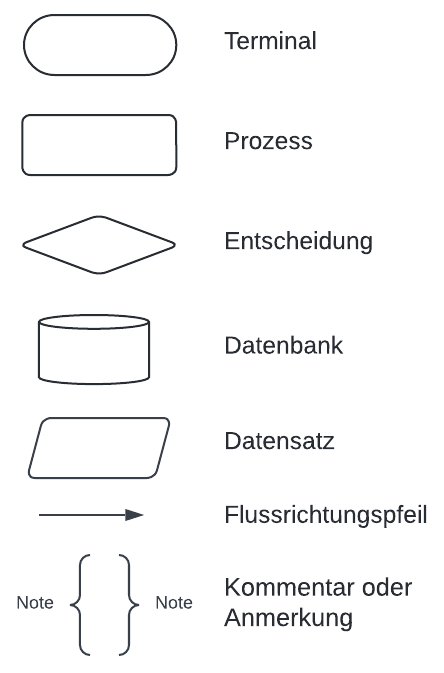
\includegraphics[height=6.5cm]{figures/flowdiagram}
 	\caption[Formen eines Flussdiagramms]{Formen eines Flussdiagramms.}
 	\label{fig:flowdiagramappen}
 \end{figure}
